\documentclass{beamer}
\batchmode
\usepackage{graphicx}
\usepackage{animate}
\usepackage{hyperref}
\usepackage{framed}
\usepackage{blindtext}
\usepackage{multicol}
%导入一些用到的宏包
\usepackage{amsmath,bm,amsfonts,amssymb,enumerate,epsfig,bbm,calc,color,ifthen,capt-of,multimedia,hyperref}
\usepackage{wrapfig}
\usepackage{subfig,graphicx}
\usepackage{xeCJK} %导入中文包
\setCJKmainfont{SimHei} %中文字体采用黑体  Microsoft YaHei

%设置Beamer主题
\usepackage{hyperref}
\usetheme{AnnArbor} %主题
\usecolortheme{beaver} %主题颜色
%代码设置
\usepackage{fancybox}
\usepackage{xcolor}
\usepackage{times}
\usepackage{listings}

\definecolor{mygreen}{rgb}{0,0.6,0}
\definecolor{mygray}{rgb}{0.5,0.5,0.5}
\definecolor{mymauve}{rgb}{0.58,0,0.82}
\newcommand{\Console}{Console}
\lstset{ %
	backgroundcolor=\color{white},   % choose the background color
	basicstyle=\footnotesize\rmfamily,     % size of fonts used for the code
	columns=fullflexible,
	breaklines=true,                 % automatic line breaking only at whitespace
	captionpos=b,                    % sets the caption-position to bottom
	tabsize=4,
	commentstyle=\color{mygreen},    % comment style
	escapeinside={\%*}{*)},          % if you want to add LaTeX within your code
	keywordstyle=\color{blue},       % keyword style
	stringstyle=\color{mymauve}\ttfamily,     % string literal style
	% numbers=left, 
	%	frame=single,
	rulesepcolor=\color{red!20!green!20!blue!20},
	% identifierstyle=\color{red},
	language=c
}
\title{面向数据驱动编程的解释器的设计与实现}
\subtitle{\fontsize{9pt}{14pt}\textbf{Moneky解释器的实现过程}}
\author{}
\institute{}
\date{\today}
\begin{document}
	\maketitle
	\setlength{\parindent}{2em}
    \section{词法分析}
    \begin{frame}
        \frametitle{词法分析概述}

        词法分析实际上的作用是将原本并无意义的字符串(我们的输入)转化为词素,生成并输出一个个词法单元。

        不仅仅是一门语言需要用到词法分析,实际上我们在更多地方都能看见它,比如我们的数据库,SQL语句其实也是一个个的词素的组合,
        
        还有其他可交互平台中,我们在Shell中的输入,实际上也同样会被转化为对应的词法单元,然后再通过语法分析,最后再交由机器执行。

        所以词法分析其实就相当于我们阅读文言文的时候,是不是会对大部分的词语进行标注,从而才能为接下来翻译的过程做好准备。
    \end{frame}
    \begin{frame}
        \frametitle{词法单元}
        \begin{columns}
		\column{0.5\textwidth}
		
        有了先前的描述,我们已经对词法分析有了一定程度的了解,接下来不妨让我们看看我们要设计的语言的基础模样。
		
		\column{0.5\textwidth}
		\centering
		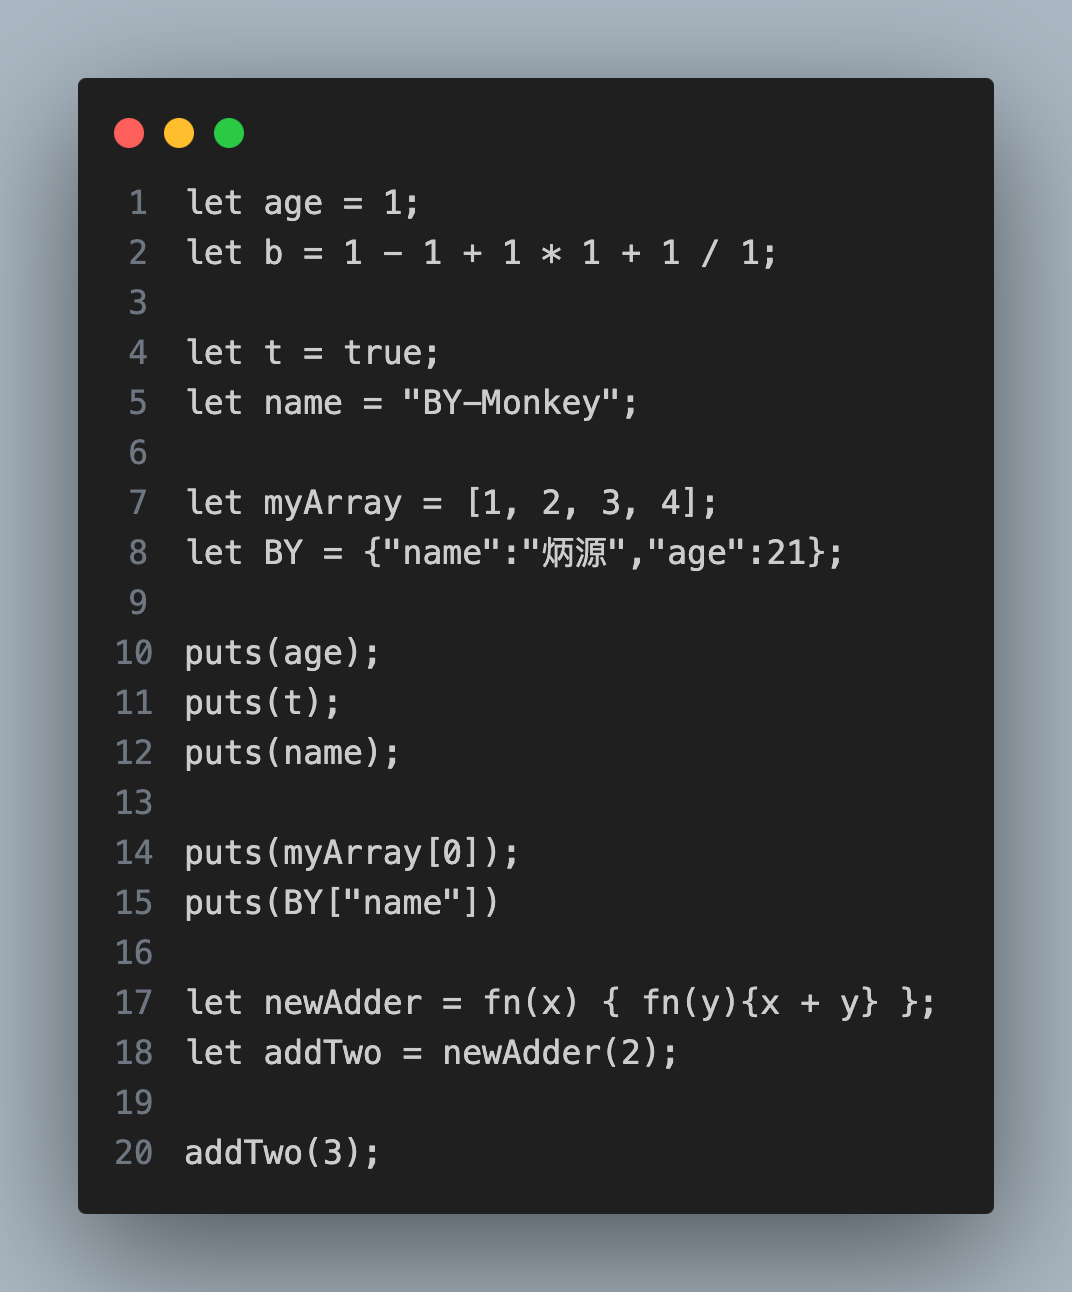
\includegraphics[width=0.95\textwidth]{pics/code0-0}
		\end{columns}
    
        
    \end{frame}
    \begin{frame}
     刚刚展示的代码中,我们能够大体把遇到的词法单元分为以下几类:

        \begin{itemize}
            \item 操作符:`+,-,*,/,=`
            \item 标识符,也就是我们的变量名和函数名,我们把他们归为一类
            \item 关键字:`let,fn`
            \item 内置函数:`puts`上述例子中只展示了这一个内置函数,不过没事,我们会逐步添加的!
            \item 特殊字符:`(,),[,],{,},:,EOF`
            \item 字面量:字面量即`1234`,`"1234"`,`ture`这类数值or字符串,他们也是我们词法单元的一类
        \end{itemize}

        而我们词法分析的目的,就是将其一个个从原本的输入中摘出来,并标注清楚。
    \end{frame}

    \begin{frame}
        有了各个确定的词法单元,我们接下来就定义一下基础的词法分析器结构:

        \centering
        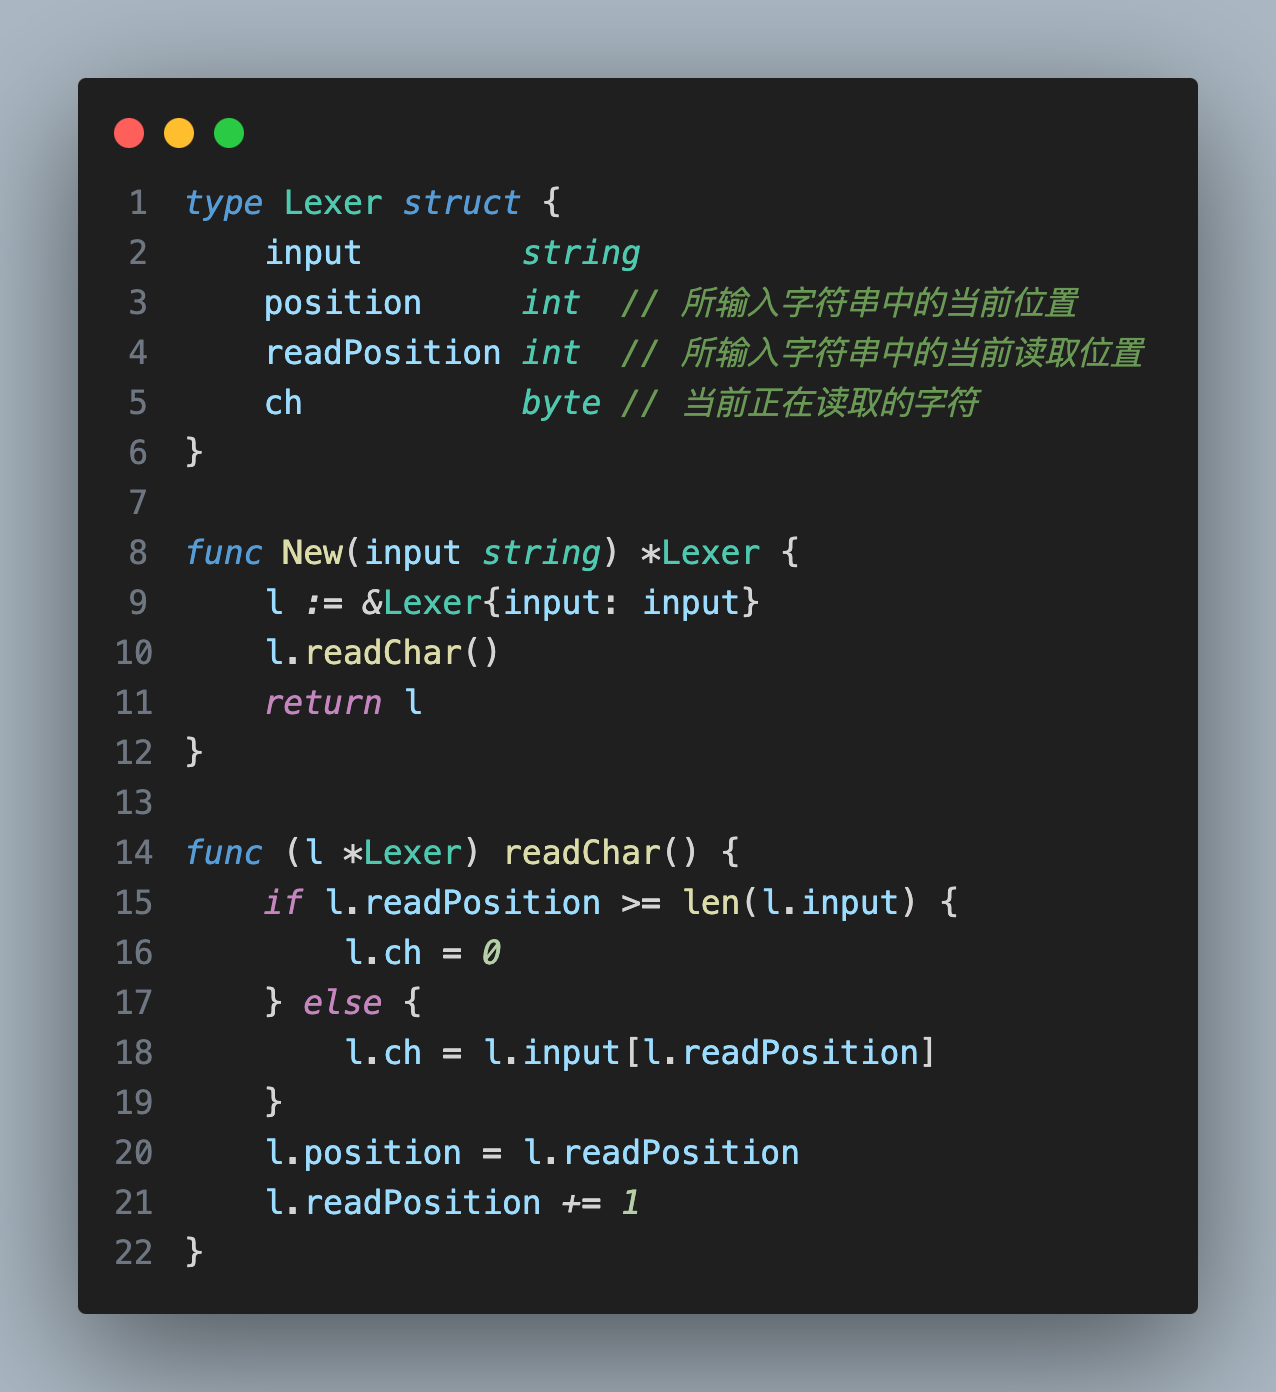
\includegraphics[width=0.5\textwidth]{pics/lexer}
    \end{frame}
    \begin{frame}
        首先`input`是我们正在处理的整段代码,`position`则是我们正在分析的位置,
        `readPosition`则是一个类似于缓冲区的位置,是我们已经读取但是还没有分析的位置,我们可以通过这个来实现“偷窥”下一个字符的功能,从而能够更好地判断当前的词法单元是什么。

        但是它现在的能力还不足以识别词法单元。我们还需要对其进行完善,我们继续来编写一个`nextToken()`函数,这个函数能够返回当前正在阅读的词法单元。
        
        我们还是从比较简单的情况开始吧。首先我们来尝试识别一下括号和加减乘除。
    \end{frame}
    \begin{frame}
        \begin{columns}
    		\column{0.5\textwidth}
    		
            首先是`skipWhitespace()`这个函数,我们稍微看一下便能明白其功能,就是将空格和换行等等我们并不需要的部分直接跳过,毕竟,我们作为人看代码才更需要可读性,而对于词法分析器来说,只需要挨个阅读过去即可。

            然后则是`NextToken()`,我们在这个函数中才真正实现了读取并加上“注释”的这一功能,其实这一宏大的功能这样子一看,并不是那么难以理解。
            
            我们对于当前`lexer`正在解析的字符进行判断,并把不同种类的括号与运算符和他们对应的词法单元,然后返回对应的`Token`,便完成了标注。
    		
    		\column{0.5\textwidth}
    		\centering
    		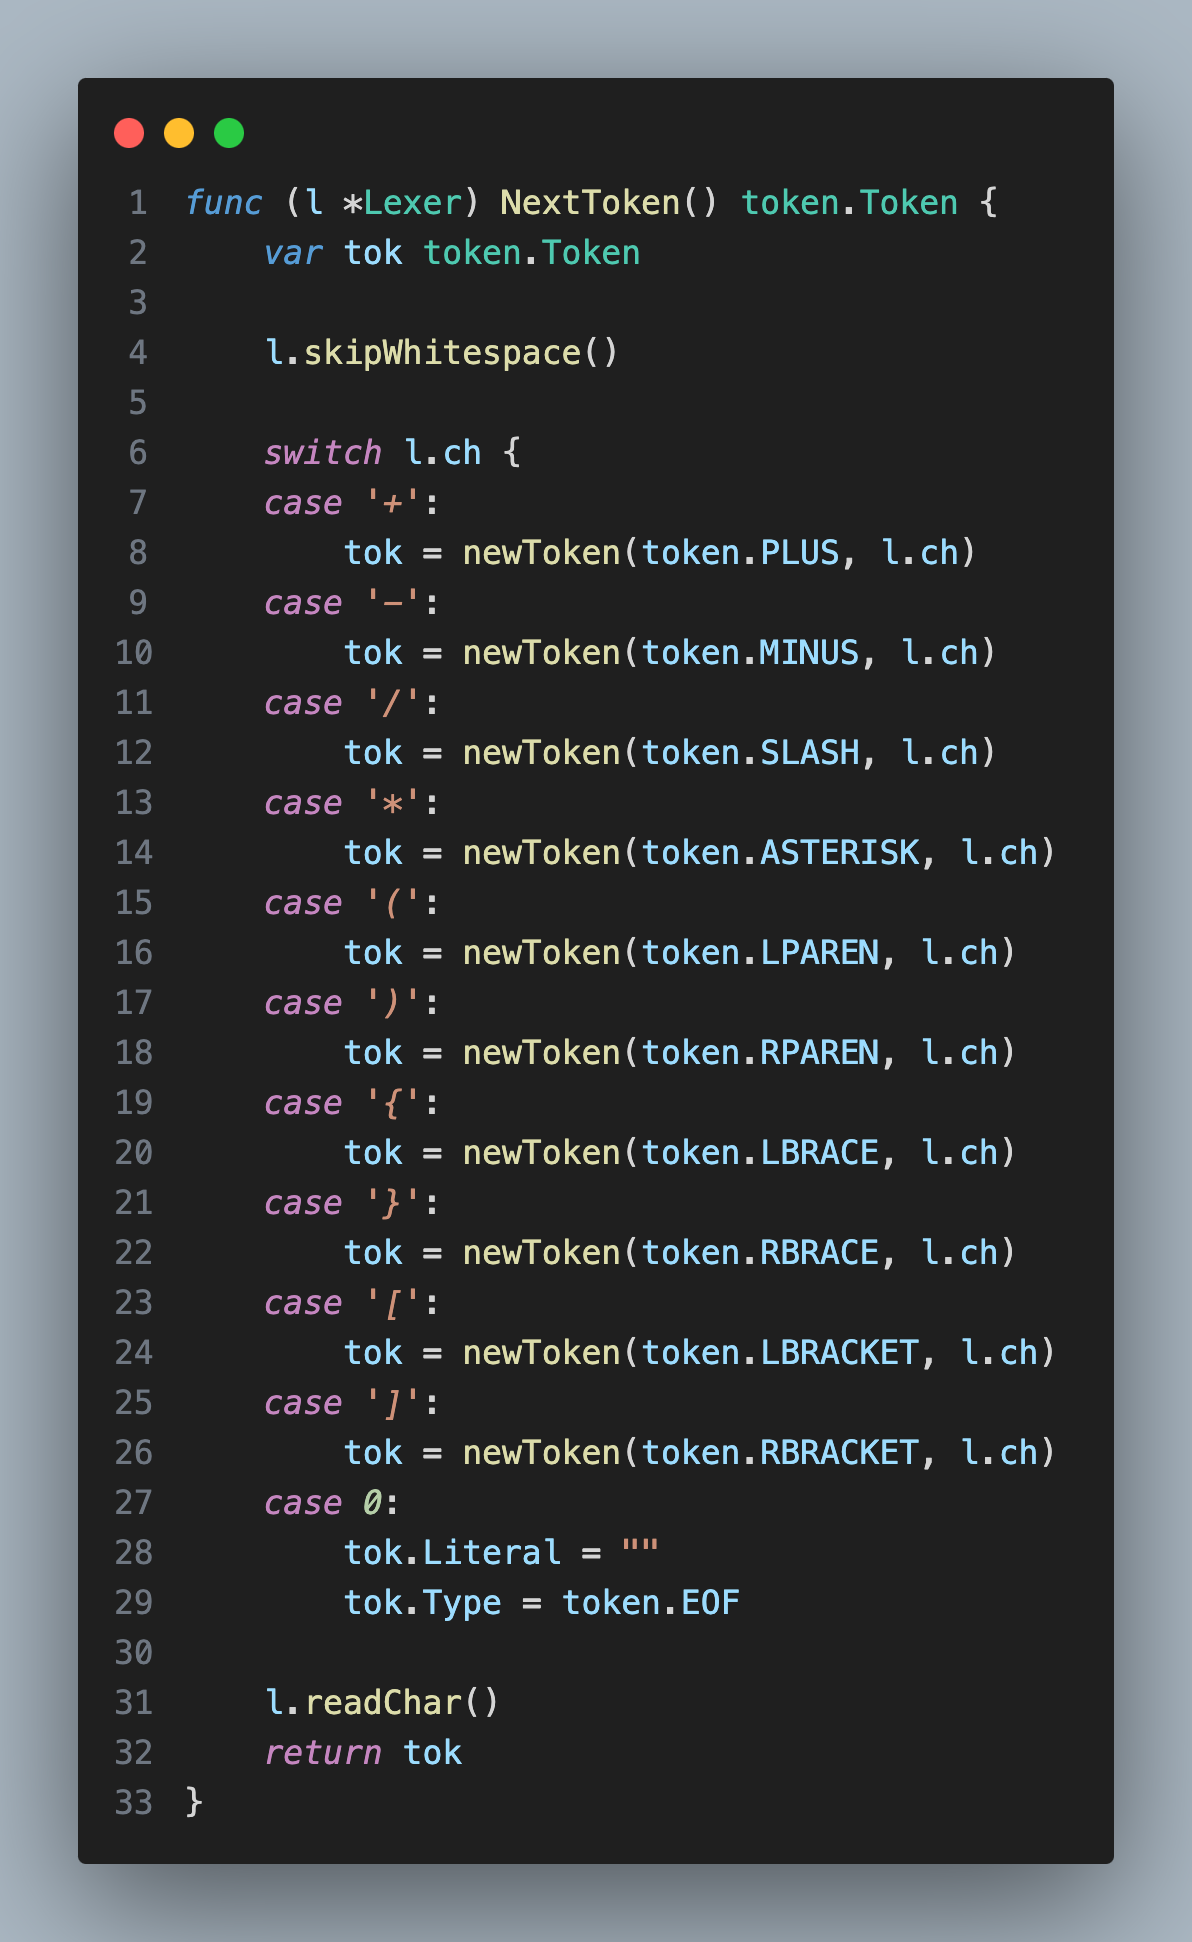
\includegraphics[width=0.85\textwidth]{pics/nextToken}
		\end{columns}
    \end{frame}
    \begin{frame}
        但是还有另外一个棘手的问题出现了,按照我们刚刚的`lexer`的逻辑,我们得在`switch`中添加一个分支来识别`let`。

        可是我们只能识别一个字符!
        
        而且这个问题还必须解决,因为我们基本上所有的关键字,都并非单个字符,所以我们没办法在`case`对`l`这个字符单独识别,然后看看之后几个是不是`et`吧。
        
        同时我们还有例如`==、!=`等符号不仅仅由一个字符组成,所以我们就必须得对其进行特殊处理。
        
        于是我们引入了`peekChar()` 用于偷窥下一个字符的函数,有了这个函数,在遇到`=`、`!`时,我们就可以通过调用这个函数,从而判断它是否属于`==`和`!=`的情况了。
        
        但是对更多的字符的关键字,我们就没办法通过`peekChar()`来解决了,所以我们只能对`default`分支做手脚。
        
        我们先编写一个`map`用于存放我们的关键字,不仅仅是`let`,还有其他的我们所需要用到的关键字。
    \end{frame}
    \begin{frame}
        \centering
        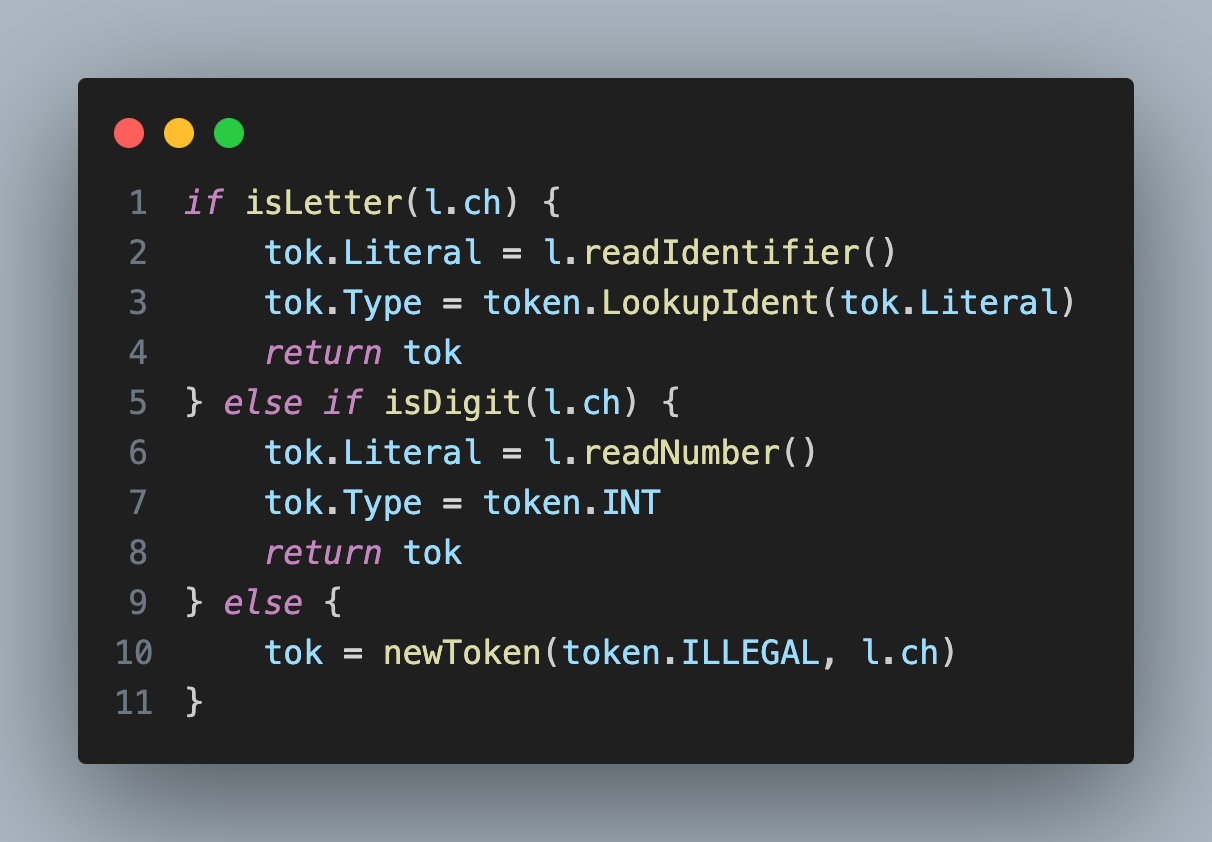
\includegraphics[width=0.85\textwidth]{pics/lexerDefault}

        而最终,我们NextToken函数的 default 分支的部分就如同这样子了。
    \end{frame}
    \begin{frame}
        首先如果我们遇到的是字母字符,则它大概率是个字面量or关键字,所以我们将其读取直到 遇到第一个非字母/数字字符。这样子我们对于BY-Monkey语言的变量声明就有了一个基础的规定—— 禁止以数字开头 !!!
        
        接着再将其放入刚刚的`keywords`,看其是否在其中,就可以将其从变量与关键字分开。
        
        其次如果我们遇到的是数字字符,则它大概率是个数字,我们就一直读取到第一个非数字字符即可停止。
        
        完成了上述两个,如果还有其他的,那么就只剩下非法的情况了。        
    \end{frame}
    \section{语法分析}
	\begin{frame} 
		\frametitle{语法分析概述}
		
		语法分析器需要检查词法分析器输出的词法单元序列是否合法,并且以该词法单元序列生成对应的抽象语法树。
		
		一个比较简单理解的概念就是—— \textbf{JSON解析器}
		
		看下面这一段js代码\textsuperscript{[1]}:
		
		\lstinputlisting[lastline=8,
		language=JavaScript,
		frame=single]
		{./code/json.parse().js}
    \end{frame}
	\begin{frame}
		
		刚刚的内容是一段来自MDN的代码,对应的内容则是:
		
		\begin{quote}
			JSON.parse() 方法用来解析 JSON 字符串,构造由字符串描述的 JavaScript 值或对象。提供可选的 reviver 函数用以在返回之前对所得到的对象执行变换 (操作)。
		\end{quote}
	
		所以$parse()$函数做的就是检查原本无意义的意义的字符串是否符合json规范,并转化为对应的js值或者对象。
		
		
		我们语法分析器要做的也是如此,只不过有了之前词法分析的帮助,我们不需要直接面对无意义的字符串,而是可以面对带有 “字典注释” 的词法单元。
		
		但即便如此,我们这一步的任务还是颇为艰巨,毕竟我们这一步就要补充我们这门语言的语法标准了,工作量还是有的。
		
	\end{frame}

	\begin{frame}
		而产生的抽象语法树又有什么作用呢?
		
		按照抽象语法树,我们可以选择自己对应语法的遍历顺序,依次遍历并求解对应的值——最后的结果就是代码执行的结果了,这就是下一节——求值系统需要做的事情了。
		
		说到如此,可能还是有些抽象,我们不妨来直观感受一下抽象语法树到底是个什么东西。
		
		\lstinputlisting[lastline=8,
		language=js,
		frame=single,
		label=js]
		{./code/try.js}
	\end{frame}
	\begin{frame}
		
		\begin{columns}
		\column{0.5\textwidth}
		上述代码很简单,我们一眼就能看出其执行结果和含义,而它所产生的抽象语法树(可能的形式之一),我们可以这样子来表示:
		
		\column{0.5\textwidth}
		\centering
		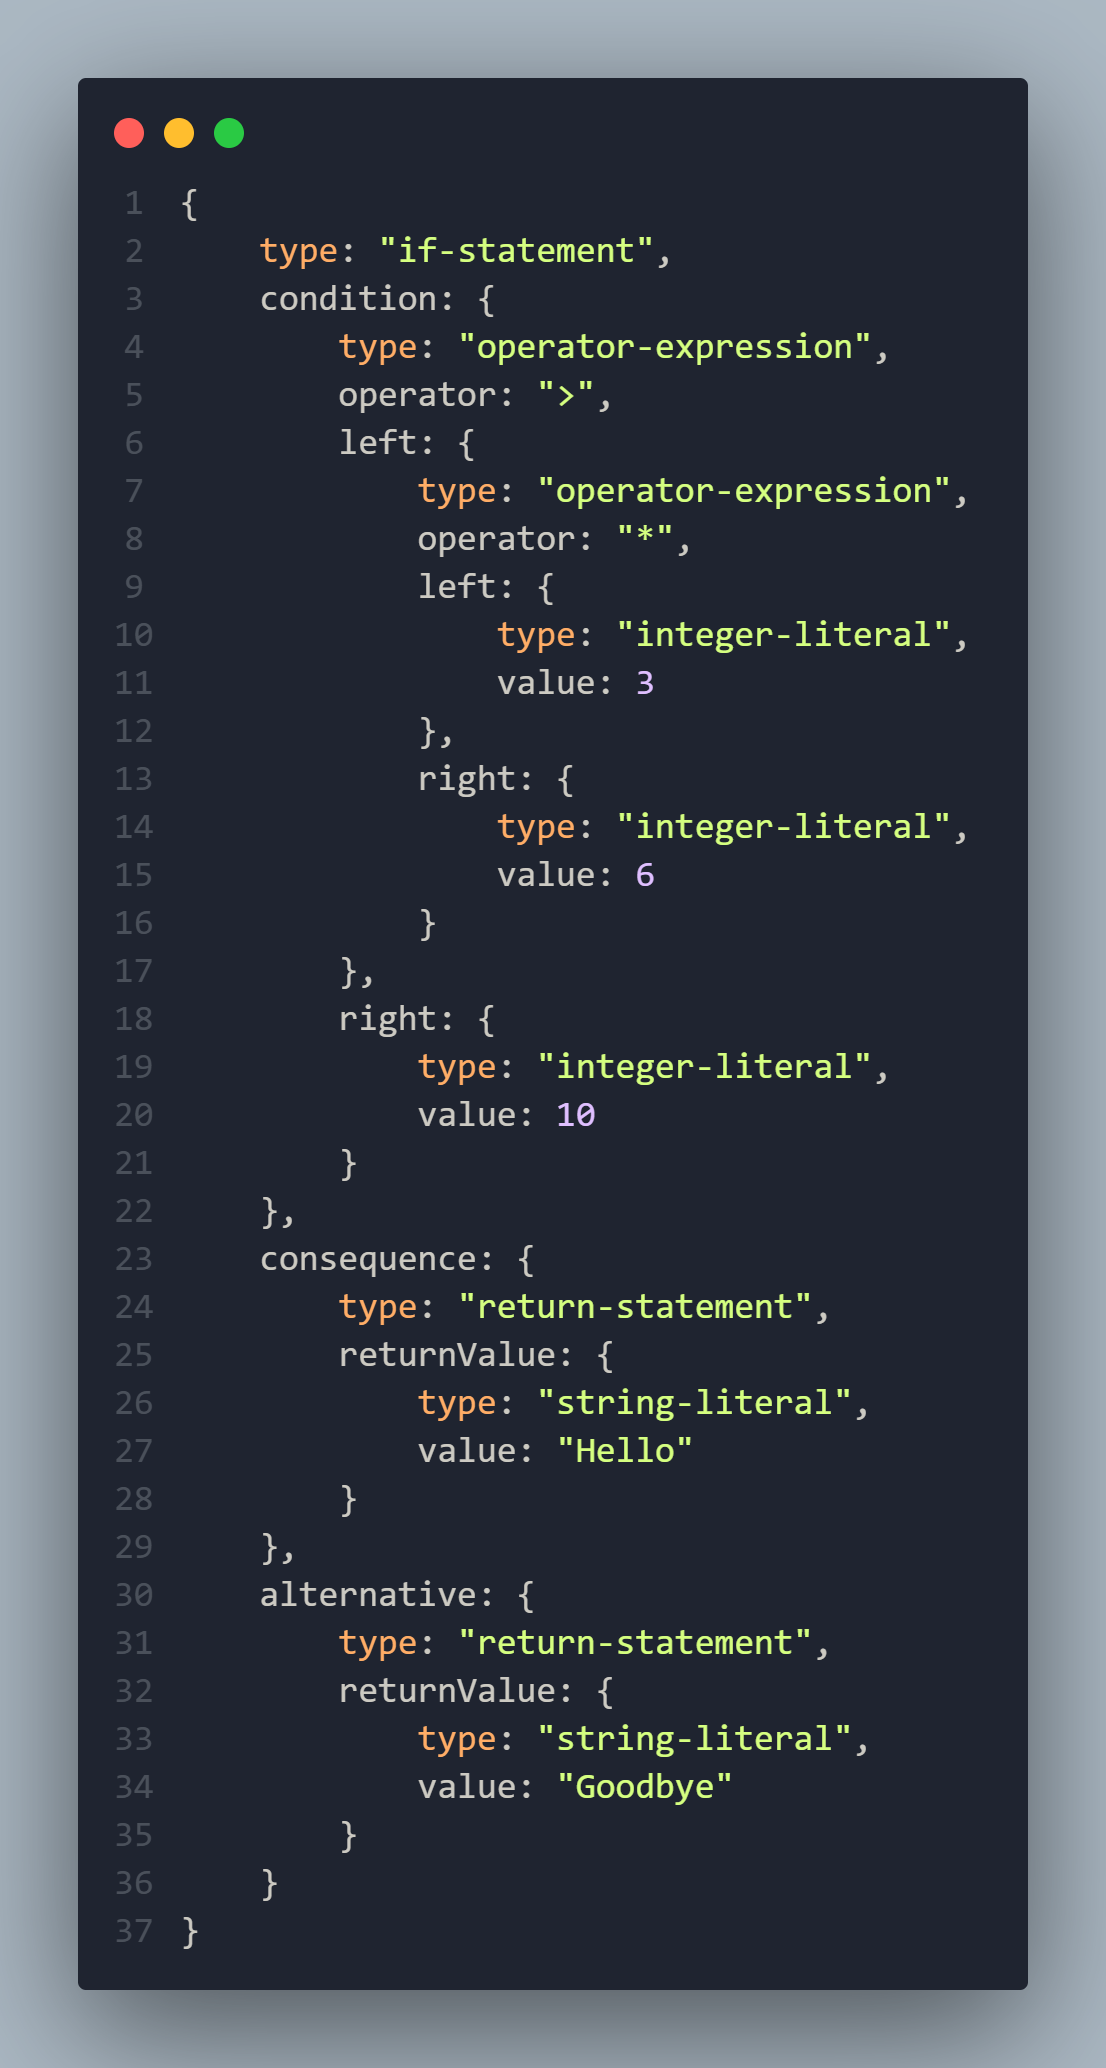
\includegraphics[width=0.75\textwidth]{pics/code1}
		\end{columns}
	\end{frame}
	\begin{frame}
		还是觉得抽象?我们可以来看看所对应的结构图:
		
		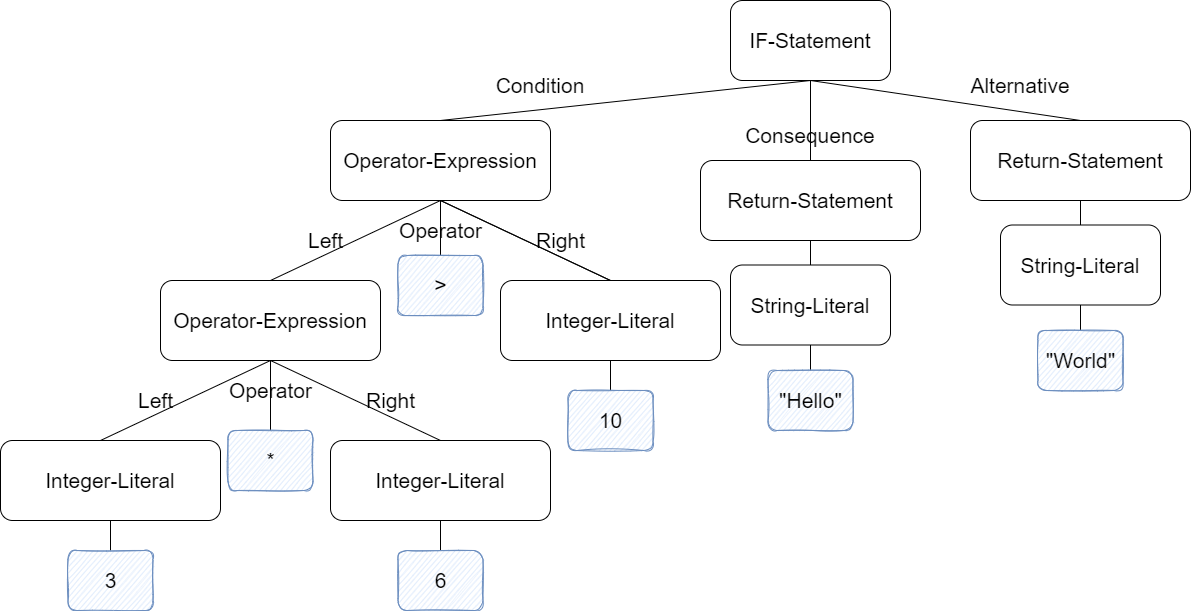
\includegraphics[width=0.8\textwidth]{pics/抽象语法树}
		
		这下子就能很直观的看到了我们要构建的抽象语法树了,化抽象为直观,才能方便我们理解我们接下来的工作。
	\end{frame}
	\section{LL(1)文法与递归下降分析法}
	
	\begin{frame}
		\frametitle{LL(1)文法与递归下降分析法}
		对于被称为 LL(1) 的文法,我们可以构造出预测分析器,即不需要回溯的递归下降语法分析器。
		
		\begin{quote}
			LL(1)文法:从左向右扫描输入,产生最左推导,每一步只需要向前看一个输入符号来确定语法分析动作
		\end{quote}
		
		
		不同于自下而上的语法分析器,自上而下的递归下降分析法是从构造AST的根节点开始,然后下降。
		
		而要实现这个分析器,我们所要做的第一步,就是确定构成我们的抽象语法树的数据结构。
		
		让我们这次从一个比较简单的例子实践入手
	\end{frame}
	
	\section{解析 let 语句}
	\begin{frame}
		\frametitle{解析 let 语句}
		我们从简单的语句开始入手构建我们的抽象语法树,因为是树状结构,所以我们可以每个部分都依次编写好对应的模块,然后再组合在一起。
		
		我们再来回顾一下我们的BY-Monkey语言的let语句:
			
		\lstinputlisting[lastline=8,
		language=python,
		frame=single,
		label=python]
		{./code/let.txt}
		
		
		上面的语句稍微总结一下,其实我们会发现,可以总结为以下的形式:

		let <ident> = <expression>
		
		
		即 "let 标识符 = 表达式" 的形式,我们用它来声明变量,用来定义函数。
	\end{frame}
	\begin{frame}
		
		而接下来,我们需要明确一下 \textbf{语句} 和 \textbf{表达式} 之间的区别:
		
		\begin{itemize}
			\item 语句不产生值
			\item 表达式产生值
		\end{itemize}
		
		例如`let x = 5`并不会产生值,而`3 + 6`会产生值。
		
		
		我们的AST就是由语句结点和表达式结点来构成的,所以我们可以得到AST的数据结构的初始定义:
	\end{frame}
	\begin{frame}	
		\lstinputlisting[lastline=20,
		language=python,
		frame=single]
		{./code/node.txt}
		
		
		这里有三个接口,AST中的每个结点都需要实现Node接口,也就是必须实现TokenLiteral()方法和String()方法,
		分别返回与结点关联的词法单元的字面量和其格式化的结构输出(用于Debug比较)。
		
		我们将要构建的AST是一棵由许多相互相互连接的结点组成的树,有些结点实现了Statement接口,有些结点实现了Expression接口。
	\end{frame}
	\begin{frame}
		我们先来实现一个Program \textbf{结点} ,因为我们的分析的的根节点,自然是一个包含了许多语句的代码,而且它也方便理解。
		
		\lstinputlisting[lastline=20,
		language=python,
		frame=single]
		{./code/program.txt}
		
	\end{frame}

	\begin{frame}
		上述的代码中,我们实现了Program结点,它的TokenLiteral()方法,会返回这段代码块的第一个的语句结点的字面量。
		
		现在再来看看我们的let语句,我们就能差不多拟出一个类似的结构来将我们先前说的let <ident> = <expression>这个形式的抽象语法树的子树给构建起来。
		
		让我们先构建一下其子树大概的样子:
		
		\begin{figure}[h]
			\centering
			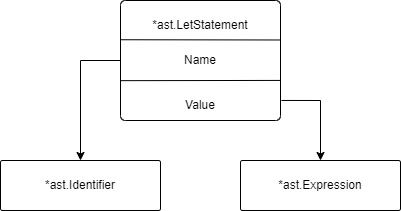
\includegraphics[width=0.6\textwidth]{pics/letStatement}
		\end{figure}
	\end{frame}

	\begin{frame}
		有了这个子树大概模样,我们很快就能构建出其对应的数据结构:
		
		\lstinputlisting[lastline=20,
		language=python,
		frame=single]
		{./code/letStatement.txt}
	\end{frame}

	\begin{frame}
		而有了对应的抽象语法树结点,我们的任务就是构建出能将词法单元组织成上述抽象语法树的一个\textbf{语法分析器}了。
		
		\lstinputlisting[lastline=20,
		language=python,
		frame=single]
		{./code/parser.txt}
	\end{frame}
	\begin{frame}
		上述的Parser中,l是我们在前面词法分析的词法分析器,errors是我们在语法分析中遇到不符合语法的错误
		
		curToken则是我们正在解析的词法单元,peekToken则是我们下一个要解析的词法单元,prefixParseFns和infixParseFns则是我们后面遇到不同的表达式/不同的词法单元所需要用到的对应解析函数(我们后面马上会提到)。
		
		接下来就是我们解析器的入口函数了
		
	\end{frame}
	\begin{frame}
		还记得我们先前提到的Program结点吗?
		
		它是我们整个程序的入口,所以自然解析函数的首要就是解析它:
		
		\lstinputlisting[lastline=20,
		language=python,
		frame=single]
		{./code/parseProgram.txt}
	\end{frame}
	\begin{frame}
		上述的代码是我们Parser的一个方法,它会返回一个*ast.Program,我们在下一步的——对象求值系统,也是通过它来开始的。
		
		观察到上面我们的parseStatement方法,这其实就是递归下降分析法的体现了,具体来说就是根据当前词法单元来决定调用哪些函数构造AST结点。而且这些函数都可以互相递归调用。
		
		ParseProgram()的执行过程,首先是先构造AST的根节点,也就是我们的*ast.Program,然后遍历输入中的每个词法单元,直到遇到token.EOF。
		
		如果解析语句返回的结果并非空,那么就将其添加进Statements切片(数组)。
		
		而接下来我们要观察的就是parseStatement这个函数了。
	\end{frame}
	\begin{frame}
		\lstinputlisting[lastline=20,
		language=python,
		frame=single]
		{./code/parseStatement.txt}
		
		上述的parseStatement()是个选择器,根据不同的词法单元调用不同的解析函数,这就是我们递归下降分析的重点了。
		
		而且,我们也终于到了本章的主角——parseLetStatement()
	\end{frame}
	\begin{frame}
		接下来就让我们看看这个主角到底是怎么样子的一个结构
		
		\lstinputlisting[lastline=20,
		language=python,
		frame=single]
		{./code/parseLetStatement.txt}
	\end{frame}
	\begin{frame}
		上述的方法中我们依旧是先把*LetStatement结点给建立出来,
		
		接着再依次判断其下一个词法单元是不是标识符,如果是,就继续移动词法单元,如果不是,就说明我们遇到了错误的情况,返回空,然后再将标识符对应的词法单元加入到我们的AST中。接着继续检查是不是等于号,然后再检查等号右侧是不是表达式,而最后,判断是不是分号,BY-Monkey语言并不强制加分号来结束我们的语句。
		
		这时候问题就来了,我们的错误检测和错误恢复去哪里了呢?
		
		答案是在expectPeek()中
		
	\end{frame}
	\begin{frame}
		\lstinputlisting[lastline=20,
		language=python,
		frame=single]
		{./code/expectPeek.txt}
		
		当我们预测的词法单元与实际的并不符合的时候,我们会向之前Parser结构中的errors添加一条错误信息,表明此处应该使用的词法单元和实际接收到的词法单元。
		
		如此,我们就基本完成了let语句的解析。
	\end{frame}
	\begin{frame}
		不同于《编译原理》中介绍的恐慌模式的错误恢复策略,我们采用的方法并没有忽略什么词法单元,而是基于我们的预测结果给出对应的修改建议。
		
		因为恐慌模式存在下面几个缺点:
		
		\begin{itemize}
			\item 信息不足: 在恐慌模式下,编译器可能会在遇到一个错误后立即中断编译,而没有尝试分析和修复其他可能存在的错误。这可能导致只报告了一个错误,而隐藏了其他相关的错误。
			
			\item 效率低下: 恐慌模式下,编译器可能会频繁地中断编译,导致编译过程的效率降低,特别是当程序中存在大量错误时。
			
			\item 可能错过潜在的问题: 编译器在恐慌模式下可能会错过一些潜在的问题,因为它会在遇到第一个错误时立即停止编译,而不考虑是否有其他问题也需要解决。
		\end{itemize}
	
		而我们的方法则将上述几个缺点较好的解决了。
	\end{frame}
	\section{测试代码编写}
	\begin{frame}
		\frametitle{测试代码编写}
		完成了功能的编写,接下来就是对功能的测试了
		
		\lstinputlisting[lastline=20,
		language=python,
		frame=single]
		{./code/TestLetStatement(1).txt}
	\end{frame}
	
	\begin{frame}
		\lstinputlisting[lastline=20,
		language=python,
		frame=single]
		{./code/TestLetStatement(2).txt}
		
	
	\end{frame}

	\begin{frame}
		在上面展示的代码中,我们编写了三个对应的样例。然后分别对其进行测试,先利用词法分析器将其词法单元提取出来,接着再利用ParseProgram()方法构建对应的抽象语法树,然后再检查是否有错误,如果无误,则对产生的Statements[]切片进行逐个的检验,观察是否是对应的结点。
		
		而checkParserErrors()方法也可以替我们检测那些错误的测试用例,即面对语法出现错误的情况,我们的词法分析器会抛出的错误提示。这同样也是测试的一环,碍于篇幅限制,就不在此展示重复的测试代码了。
		
	\end{frame}

	\section{解析表达式}
	\begin{frame}
		\frametitle{解析表达式}
		
		其实我们并没有很好的完成我们对于let的解析,因为等号的右侧——表达式,我们还没有处理。
		
		而这,其实是编写语法分析器中最有趣的部分。
		
		对于语句的解析过程无非就是从左到右依次处理词法单元,然后对下一个词法单元进行期望检验。
		
		但是解析表达式就不仅如此了,我们需要考虑处理运算符的优先级,以及运算符的左关联和右关联情况
		
		而解析表达式,我们依旧是使用\textbf{自上而下的运算符优先级分析法},也就是大名鼎鼎的普拉特解析法。
		即论文"Top Down Operator Precedence"中,沃恩·普拉特提出的方法。
		
		不同于我们先前使用的将解析函数(如我们的parseLetStatement)与语法规则相关联的方式(即挨个预测是不是符合我们的语法)。普拉特分析法采用了将解析函数(论文中称为semantic code)与词法单元相关联的方法。
	\end{frame}
	\begin{frame}
		来回看我们先前的Parser中是不是有两个比较奇怪的结构:prefixParseFns和infixParseFns,粗略的解释仍然不能将他们两个的意思阐明。
		
		他们两个对应的分别是普拉特论文中的"nuds"和"leds",用比较直观的例子来解释,比如- -i,就是利用prefixParseFns里面的方法来解析的,因为其代表的是前缀运算符,而像3 + 5这个例子来说, + 代表的则是中缀运算符,就需要调用infixParseFns里面的方法来解析,我们来看看prefixParseFn和infixParseFn两个类型的原型:
		
		\lstinputlisting[lastline=20,
		language=python,
		frame=single]
		{./code/ParseFn.txt}		
	\end{frame}
	\begin{frame}
		可以看到,prefixParseFn是一个返回ast.Expression结点的函数类型,而infixParseFn则是一个接受ast.Expression并返回ast.Expression结点的类型,为什么会有这样子的不同呢?
		
		而prefixParseFns和infixParseFns则是token对应的前缀运算符解析函数和中缀运算符解析函数的映射。
		
		因为中缀表达式带有左值和右值,我们一般阅读到中缀运算符的时候,是已经将其运算符左边的值读取到了,这时候就需要将其一起考虑进去。
		
		其实当然也有对应的后缀运算符,但是为了方便,就不再额外阐述,BY-Monkey语言也并没有额外的后缀运算符。
		
		分清楚了前缀运算符和后缀运算符,我们还有一个问题需要解决——\textbf{运算符优先级},比如5 + 5 * 10的结果是55而并非100。
		
		所以搞清楚了这些基础概念,我们就可以来着手编写我们的代码了。
	\end{frame}
	\begin{frame}
		标识符和整数字面量应该可以算是表达式里最简单的了,我们先来搞定他们。
		
		首先的是标识符,我们如果遇到的是标识符,因为它并没有什么额外的运算符,所以我们先把它的解析方法归入prefixParseFns里面,而解析标识符要做的事情也非常简单,只需要将当前词法单元以及其字面量提供给*ast.Identifier的Token和Value字段,然后返回这个结点就可以了:
		
		\lstinputlisting[lastline=20,
		language=python,
		frame=single]
		{./code/parseIdentifier.txt}	
		
	\end{frame}
	\begin{frame}
		和标识符一样,整数字面量也是表达式,它所产生的值就是整数本身,所以我们要做的也很简单,那就是将整数字面量的词法单元以及值填充对应的*ast.IntegerLiteral(即整数字面量对应的抽象语法树结点)。
		
		\lstinputlisting[lastline=20,
		language=python,
		frame=single]
		{./code/parseIntegerLiteral.txt}
		
		在这一步使用不同的整数转换函数结合先前的整型词法单元的识别,就可以表达出其他进制,但限于篇幅,就不在此体现了。
	\end{frame}
	\begin{frame}
		完成了这两个,我们再来上点稍微有难度的解析——即真正的前缀运算符的解析。
		
		BY-Monkey语言中有两个前缀运算符:!和-,其结构也一目了然:
		
		<前缀运算符><表达式>
		
		我们首先来定义ast.PrefixExpression结点:
		
		\lstinputlisting[lastline=20,
		language=python,
		frame=single]
		{./code/PrefixExpression.txt}
		
		我们可以看到,它带有对应的词法单元,操作符以及右值,所以我们也称前缀表达式为一元表达式。
		
		有了这个,我们就可以构建对应的解析函数了。
	\end{frame}
	
	\begin{frame}
		不同于标识符和整形字面量只涉及到一个词法单元,前缀表达式至少涉及两个词法单元,我们要做的不仅仅是将当前的词法单元填充进上述的Token中,还需要移动我们的curToken,然后将右值(表达式)填充进Right中。
		
		\lstinputlisting[lastline=20,
		language=python,
		frame=single]
		{./code/parsePrefixExpression.txt}
	\end{frame}

	\begin{frame}
		有个比较陌生的函数出现了——parseExpression(优先级),它是我们总的表达式解析函数,与之相关的则是优先级的选择,我们解析表达式的时候,总要根据不同的符号确定不同的优先级来让我们的表达式能解析出正确的结构。
		
		下面是BY-Monkey语言的优先级:
		
		\lstinputlisting[lastline=20,
		language=python,
		frame=single]
		{./code/precedence.txt}
	\end{frame}

	\begin{frame}
		完成了对于前缀表达式以及之前的标识符和整数字面量的解析,我们的普拉提分析法现在终于有点雏形了。
		
		接下来还剩中缀表达式,有了前面的铺垫,我们也可以比较容易容易看出它的结构:
		
		<表达式><中缀运算符><表达式>
		
		其对应数据结构也可以很快的写出来:
		
		\lstinputlisting[lastline=20,
		language=python,
		frame=single]
		{./code/InfixExpression.txt}
	\end{frame}
	
	\begin{frame}
		其对应的解析函数也和之前解析前缀表达式的类似:
		
		\lstinputlisting[lastline=20,
		language=python,
		frame=single]
		{./code/parseInfixExpression.txt}
		
		上述的代码中,我们的流程差不多是先完成了对于左值表达式的解析,然后读取下一个词法单元,发现是中缀运算符,然后调用该中缀表达式解析函数,然后再对右值进行解析。
	\end{frame}

	\begin{frame}
		这时,熟悉的parseExpression()又出现了,我们终于要接触普拉特分析法的核心了,让我们来看看它的结构:
		
		\lstinputlisting[lastline=20,
		language=python,
		frame=single]
		{./code/parseExpression.txt}
	\end{frame}

	\begin{frame}
		我们来捋一捋上述代码描述的过程:
		
		先寻找当前Token对应的前缀解析方法,如果找不到,说明是未识别的标识符,添加错误并返回空即可。
		
		接着就是解析左值,左值解析完,如果并非结束符,且下一个的优先级更高,则解析下一个Token,直到遇到优先级更小的运算符为止。
		
		因为优先级更小的运算符,就不会黏住我们当前的运算符了。
		
		最后,返回重复解析的左值即可。
		
		不同于要频繁改写文法消除左递归的传统方法,普拉特分析法更加巧妙的利用了优先级解决了左递归的问题(论文中称为运算符黏性,指运算符黏住了周围多少个操作数)。
		
	\end{frame}

	\section{扩展语法分析器}
	\begin{frame}
		\frametitle{扩展语法分析器}
		一个完备的语法分析器自然不能只有上述几个寥寥的解析方法,我们还需要实现更多。
		
		但是碍于篇幅,没办法完全详尽地阐述。
		
		这里挑一个比较有意思的点来进行说明:
		
		对于调用表达式解析函数的处理(即:add(x, y)这样子的形式),我们并不是采用什么额外的处理,而是非常巧妙地把 '(' 作为中缀表达式的运算符,
		然后左值作为调用表达式的名,右值就是参数了。
		
		比如:add(x,y),就可以把add作为左值,'('作为运算符,'x,y'作为右值即可。
		
		非常完美的解决思路,很好的套用了普拉特分析法的精髓。
	\end{frame}
	\section{求值策略}
	\begin{frame}
		\frametitle{求值策略}
		我们在先前的过程中,已经利用词法分析获得的词法序列构建起了我们的AST,或者是利用各种分析法获得了对应的产生式列表,但是他们终究还是只是将原先的字符串(源代码)转为了另外一种形式,而我们接下来的这一步,才是让原代码焕发生机的一步,这也是Monkey语言得以实现的地方。我们将根据先前步骤的各个注释,为原先的符号赋予真正能够执行的含义。
		
		而我们要构建的解释器,根据先前做的工作,我们这次要实现的是一个树遍历解释器,我们会使用语法分析器构建的AST,直接解释它,不经过任何预处理或者编译工作。这里主要还是参考了经典的Lisp解释器的实现,也主要是因为它入门
		简单,也便于之后的扩展。
	\end{frame}
	\begin{frame}
		说起来难,但是实际操作上,我们还是能比较直观地将我们要做的事情其分为两个部分:
		\begin{itemize}
			\item 遍历AST
			\item 在Go语言种表示Monkey语言中的值
		\end{itemize}
	
		下面是一个对应的伪代码,我们或许可以从中窥见我们的具体做法:
		\lstinputlisting[lastline=20,
		language=python,
		frame=single]
		{./code/1-1.txt}
	\end{frame}
	\begin{frame}
		其实这个就是我们语法制导定义里面所说的遇到综合属性和继承属性的不同处理。
		
		可以看到,我们上述的代码中,如果遇到了字面量,就直接将其值返回,如果遇到了表达式,我们则返回其对应求值的结果。
		
		而这时候我们还需要探讨一下另一个问题——我们返回的是什么?
		
		这就牵扯到,我们这个解释器要用的是什么样的内部对象系统了。
	\end{frame}
	\section{对象系统}
	\begin{frame}
		\frametitle{对象系统}
		对象系统也可以被称为“值系统”或者是“对象表示方法”。我们这个系统所要做的就是表示AST的值。这一步当然也可以加入我们的GC(Garbage Collection),垃圾回收,但是由于Go语言并不支持我们直接操作地址,我们的GC先按下不表。
		
		有些语言使用宿主语言的原生类型来直接表示所解释语言的值,有些则使用指针表示。
		
		而除了在宿主语言内部表示这些值,我们还需要向使用我们的语言的用户公开这些值及其对应的表示。
		
		例如Java为用户提供了 \textbf{原始数据类型} 如:int, byte, short, double ...。在Java的视线中,原始数据类型与其对应的原生类型密切相关,没有太多的封装,而引用类型则用于表达复合数据结构。而Ruby则大为不同,用户无权访问原始数据类型,一切皆为对象,所有的值都封装进了内部表示。
	\end{frame}

	\begin{frame}
		既然已经抛开了性能的要求,不去考虑GC,我们就直接对于遇到的每个值都用Object表示,将其封装进去。
		
		\lstinputlisting[lastline=20,
		language=python,
		frame=single]
		{./code/object.txt}
		
		其中 Type() 方法返回的是这个对象所对应的类型,即我们遇到的是int还是bool,而Inspect()方法返回的是对应值的字符串。
		
		其实这个过程有点像又回到了我们最初开始的第一步——词法分析,但是不同的是,我们这次并非对于杂乱无序的字符串进行解析,而是对于AST上的节点进行解析。
	\end{frame}

	\begin{frame}
		下面我们来看一下 Integer 类型的对应实现:
		
		\lstinputlisting[lastline=20,
		language=python,
		frame=single]
		{./code/object.Integer.txt}
		
		也很简单,里面存储的是一个int64类型,Type()方法和Inspect()方法分别也完成了他们的功能。
		
		依据类似这样子的方法,我们可以构造出布尔类型以及空类型的对应实现。
	\end{frame}
	\begin{frame}
		有了基础的种种类型我们就需要开始实现我们一开始看到的那个伪代码——Eval函数了。
		
		\lstinputlisting[lastline=20,
		language=python,
		frame=single]
		{./code/eval-1.txt}
		
		需要说明的是这个nativeBooleanToBooleanObject函数,因为我们的布尔值只可能有两种取值,如果每次遇到true或者false时都单独创建一个新的object.Boolean实在是太过于繁琐,于是我们直接使用true和false的引用来代替每次都创建新的实例,这样子就能使用这小小的改进将我们的性能提升不少。空值也是如此。
	\end{frame}
	\begin{frame}
		处理完了单个的字面量,接下来就是对应的前缀表达式和中缀表达式的求值了,其实也不难,有了之前已经处理好的AST,其实就是按照AST对应的顺序,依次分别遍历AST的左右子树,求完各自的值之后,再根据操作符对其进行对应的运算操作,最后将其的值赋予给当前的节点即可。
		
		\lstinputlisting[lastline=20,
		language=python,
		frame=single]
		{./code/eval-2.txt}
	\end{frame}
	\begin{frame}
		而要完成任务书中的操作,只需要在刚刚的步骤中添加对应的输出就可以搞定了,但是显然,我们的目标不仅仅局限于此,我们已经能支持表达式的解释了,但是还有另外一个——语句的解释,我们还没有搞定,不过没事,我们继续来解决它。
		
		其实刚刚的两份代码中,我都刻意忽略了一个地方——我们上一次提到过,我们AST的入口,也就是顶层根节点,是ast.Program,而我们的case里面并没有体现,尽管有部分原因是为了省略代码行数,方便展示在幻灯片中,但是还是得说,我们刚刚的代码是没办法直接运行的。
	\end{frame}
	\begin{frame}
		而解决方法也很简单,我们解析ast.Program就好了。
		\lstinputlisting[lastline=20,
		language=python,
		frame=single]
		{./code/eval-Statement.txt}
	\end{frame}
	\begin{frame}
		这样子,我们的解释器就有了其对应的入口了,我们也就可以利用它进行它所支持的运算操作了。
	\end{frame}
	\section{错误处理}
	\begin{frame}
		我们在之前的词法分析和语法分析阶段都实现了对应的错误处理,求值的过程当然也会遇到对应的错误,我们同样需要在这里将会出现的错误捕捉,例如:3 + true这种不合理的运算,属于是解释器没有定义的行为,我们当然要在这里对其进行错误的警告。
		
		首先,我们需要定义捕捉错误的对应结构:
		
		\lstinputlisting[lastline=20,
		language=python,
		frame=single]
		{./code/error.txt}
		
		
		这时候,我们之前在求解中缀表达式的evalInfixExpression中遇到了不清楚的运算操作,就可以直接返回newError即可。
	\end{frame}
	\section{绑定与环境}
	\begin{frame}
		\frametitle{绑定与环境}
		回到我们语法分析的开头,我们是用let词法单元开始的,这最后一个,我们来以let语句的支持为结尾,顺便说明我们的绑定功能。
		
		我们在对let语句和标识符求值的时候,需要对其中产生值的表达式进行求值,并且跟踪产生的值,这个值会被绑定到某个具体的指定名称之下,这时候就轮到我们的Environment环境登场了,它实际上是一个对于map的一个封装,我们只需要在之前的Eval中,将其也作为传入参数之一来传递即可,这样子,我们每个Eval都可以调用到对应的参数表。
	\end{frame}
     \begin{frame}
		\frametitle{References}
		
		\begin{thebibliography}{99}
			\bibitem{[1]} MDN, https://developer.mozilla.org/zh-CN/docs/Web/JavaScript/Reference/Global\_Objects/JSON/parse
			\bibitem{[2]} Vaughan R. Pratt. 1973. Top down operator precedence. In Proceedings of the 1st annual ACM SIGACT-SIGPLAN symposium on Principles of programming languages (POPL '73). Association for Computing Machinery, New York, NY, USA, 41–51. https://doi.org/10.1145/512927.512931
		\end{thebibliography}
	\end{frame}
	\begin{frame}
		\Huge{\centerline{Thank you!}}
	\end{frame}
\end{document}